\subsection{Task-Informed Data Generation for Surrogate-Based Optimization}
\label{ch6:sec:SBO}

After establishing \textit{DiffGeo}’s baseline performance, we next explore its integration into a surrogate-based optimization (SBO) workflow. In many aerodynamic design problems, engineers employ surrogate models for fast approximations of CFD simulations or experiments to optimize shapes. The training data for such surrogates is critical: it must capture the design space and relevant physics to guide the optimization effectively. Here, we investigate using \textit{DiffGeo} to sample training shapes more effectively that embed task-specific prior knowledge, and compare this approach with conventional design space exploration methods for data generation.

\subsubsection{Problem Setup}
We consider a 2D airfoil shape optimization task that maximizes the lift-to-drag ratio (L/D) of a NACA 0012 airfoil at Mach 0.85 and zero angle of attack in an inviscid flow. A geometric constraint is applied to maintain a maximum thickness of $12\%$ chord length. This setup represents a typical transonic airfoil design task. The thickness constraint $C^I_{MT}$ is implemented by evaluating the airfoil’s thickness distribution $\cT(x)$ which is the vertical distance between upper and lower surface at each chord-wise position $x$, and building an inequality energy function for any violation of the $12\%$ chord limit. Specifically, we define:
\begin{equation}
    {C^I_{MT}} = \mathop {\max }\limits_{x \in (0,1)} \left( {\left|\left|\max (0.12 - \cT(x),0)\right|\right|^2} \right)\;.
\end{equation}
$C^I_{MT}$ is nonzero only if the shape exceeds the thickness limit. 

In a typical SBO pipeline, there are two common ways to generate the surrogate’s training dataset: either (i) perturb an existing design via statistical random sampling with a low-dimensional parameterization, or (ii) collect designs from historical databases. We emulate both strategies as baselines:
\begin{itemize}
    \item \textbf{Baseline SM\#1 with Parametric Perturbations}: This strategy starts from fitting the NACA-0012 airfoil with a 15-parameter Class/Shape Transformation (CST) model to represent the airfoil’s upper and lower surfaces. Then new shapes are created by randomly sampling the CST coefficients within specified ranges using Latin Hypercube Sampling (LHS). We consider two variants of this strategy: a narrow sampling range (SM\#1-1) and a wide sampling range (SM\#1-2). For upper $\bw_u$ and lower $\bw_l$ surface coefficients, SM\#1-1 samples both coefficients between 0.1 and 2.5 times its baseline value. The trailing edge thickness $\delta_{TE}$ is varied in range of $[-10^{-3}, 10^{-3}]$. In SM\#1-2, $\bw_u$ and $\bw_l$ ranges are are expanded from 0.08 to 5 times the baseline values, producing more aggressive shape perturbations. Both SM\#1-1 and SM\#1-2 generate 500 sampled airfoils.

    \item \textbf{Baseline SM\#2 with Historical Designs}: This approach follows the practice of using data available from previous projects. To emulate this idea, a small dataset of 50 profiles randomly selected from the UIUC airfoil database is built. These represent a mix of airfoil types, such as for aircraft wings, hydrofoils, etc., many of which are not tuned for transonic $L/D$ performance. This approach is easy to implement in practice but the data collected can be misaligned with the new design objective. 
\end{itemize}

\textit{DiffGeo} provides a third approach via its conditional sampling, denoted as SM\#3. \textit{DiffGeo} is trained on the same 50-profile dataset from SM\#2, thus starting with the same information as the historical data. Despite the dataset being small and not customized for this task, \textit{DiffGeo} can learn a latent geometry distribution from it. Then the conditional generation guided by the thickness constraint produces feasible and thickness-constrained shapes, using the CLSDM coupled with the energy function $C^I_{MT}$. By sampling 500 shapes through the sampling process described by Algorithm~\ref{ch6:alg:abs_sample_conditional_diffusion}, we obtain a training set for surrogate model that is task-informed while being diverse. Fig.~\ref{ch6:fig:main_SBO_airfoils} visualizes the each resulting airfoil datasets by SM\#1-1, SM\#1-2, SM\#2 and SM\#3.

\begin{figure}[tbh]
    \begin{center}
        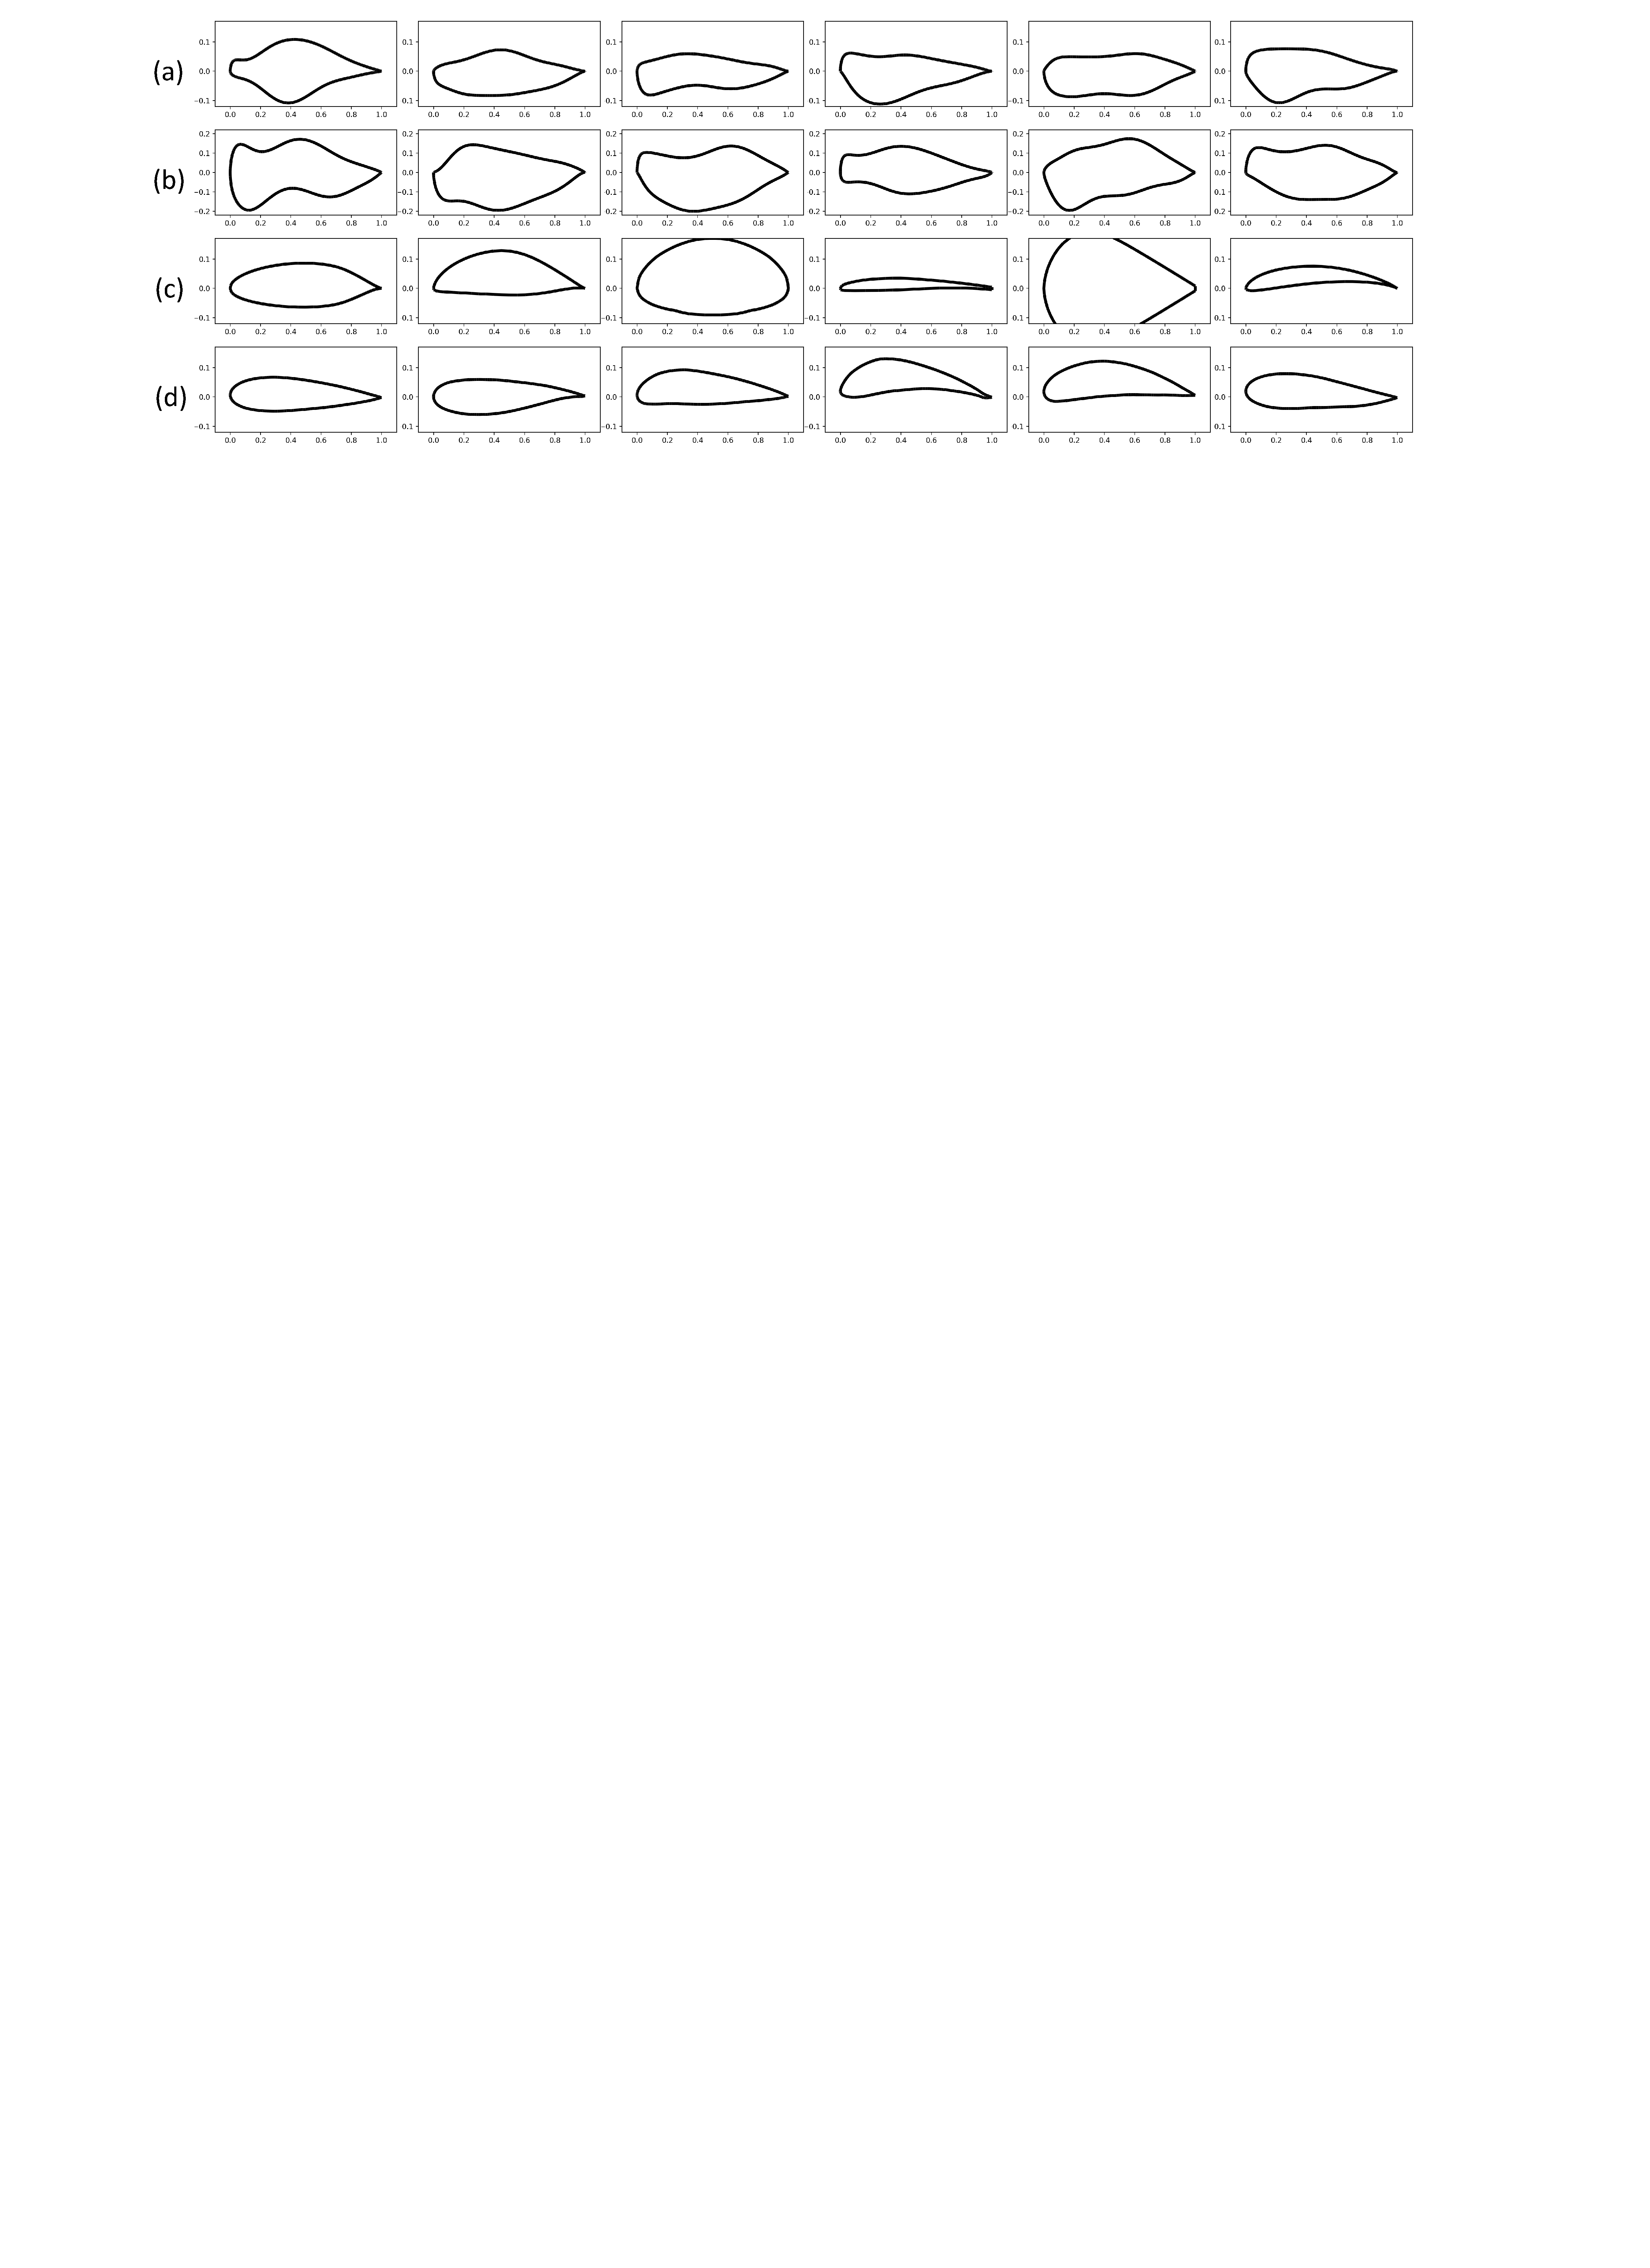
\includegraphics[width=1\linewidth]{chapter6/fig/SBO_airfoils.pdf}
    \end{center}
    \caption{
        \small Airfoil training sets: (a) SM\#1-1, (b) SM\#1-2, (c) SM\#2, (d) SM\#3. Note that (b) uses a different $y$ scale.
    }
    \label{ch6:fig:main_SBO_airfoils}
\end{figure}

\begin{figure}[!h]
    \begin{center}
        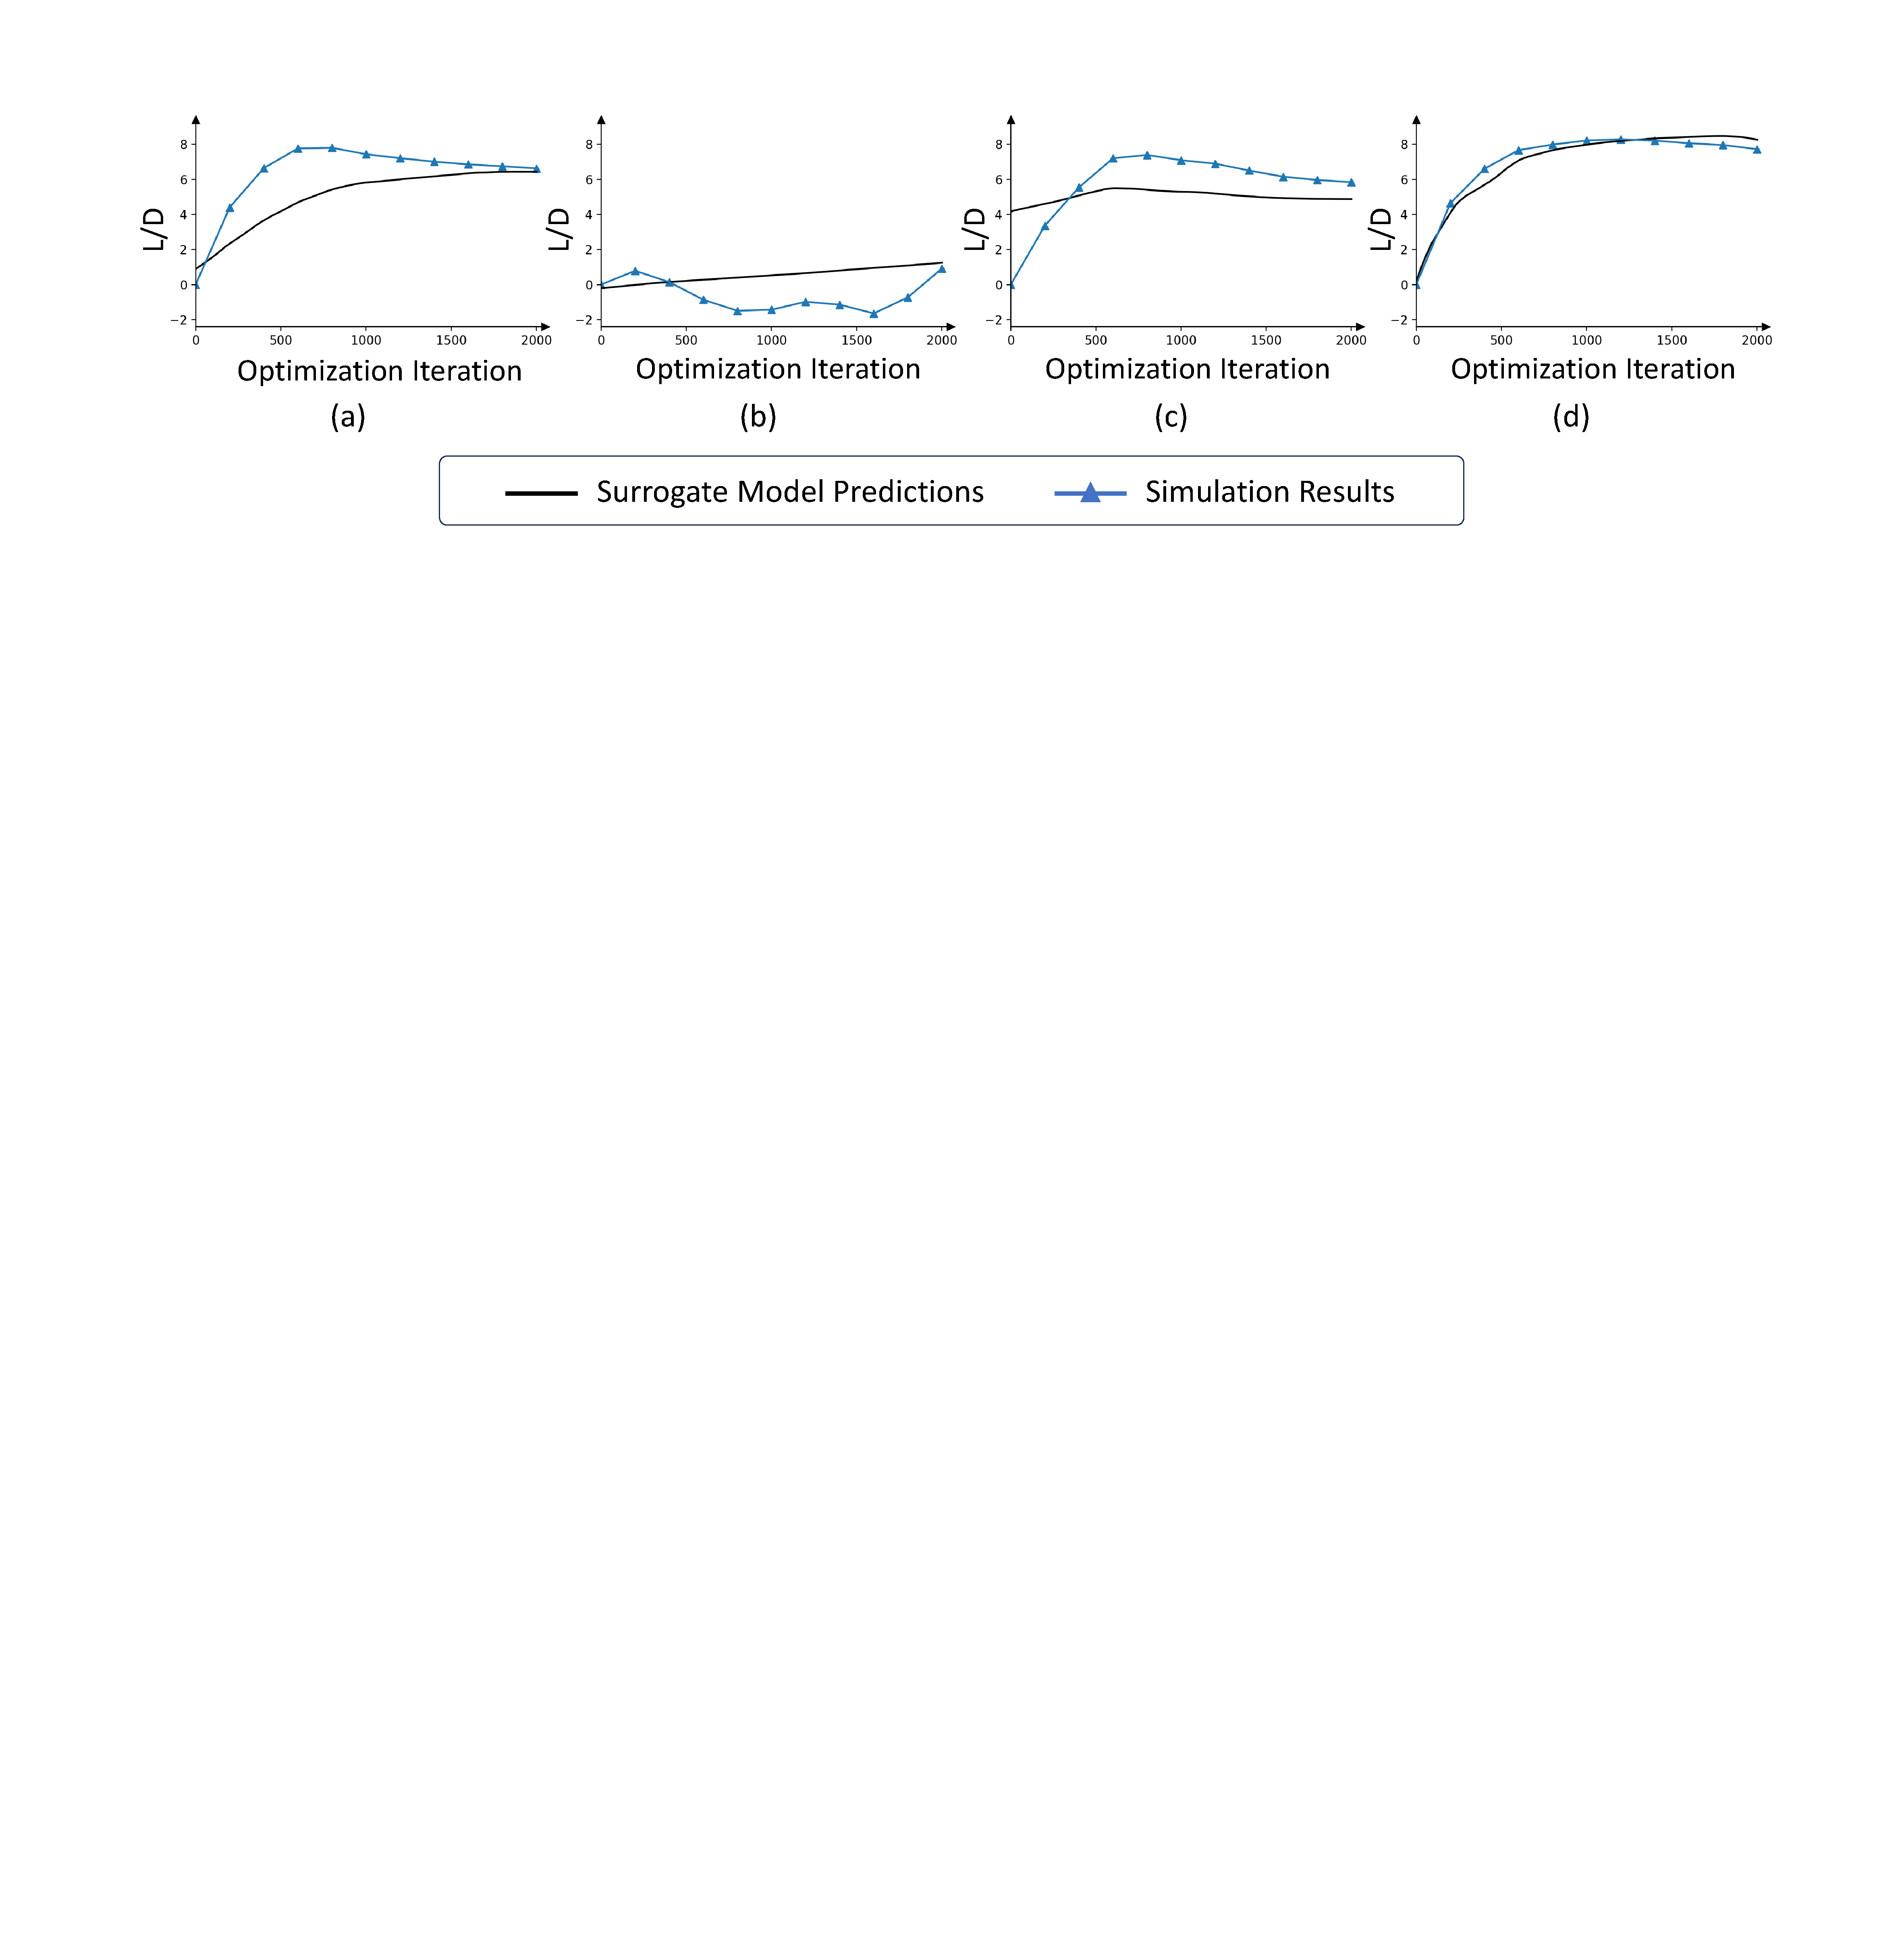
\includegraphics[width=1\linewidth]{chapter6/fig/SBO_optim_history.pdf}
    \end{center}
    \caption{
        \small Drag coefficient histories during surrogate-based optimizations with (a) SM\#1-1, (b) SM\#1-2, (c) SM\#2, and (d) SM\#3.
    }
    \label{ch6:fig:main_SBO_optimized_history}
\end{figure}

\begin{figure}[!h]
    \begin{center}
        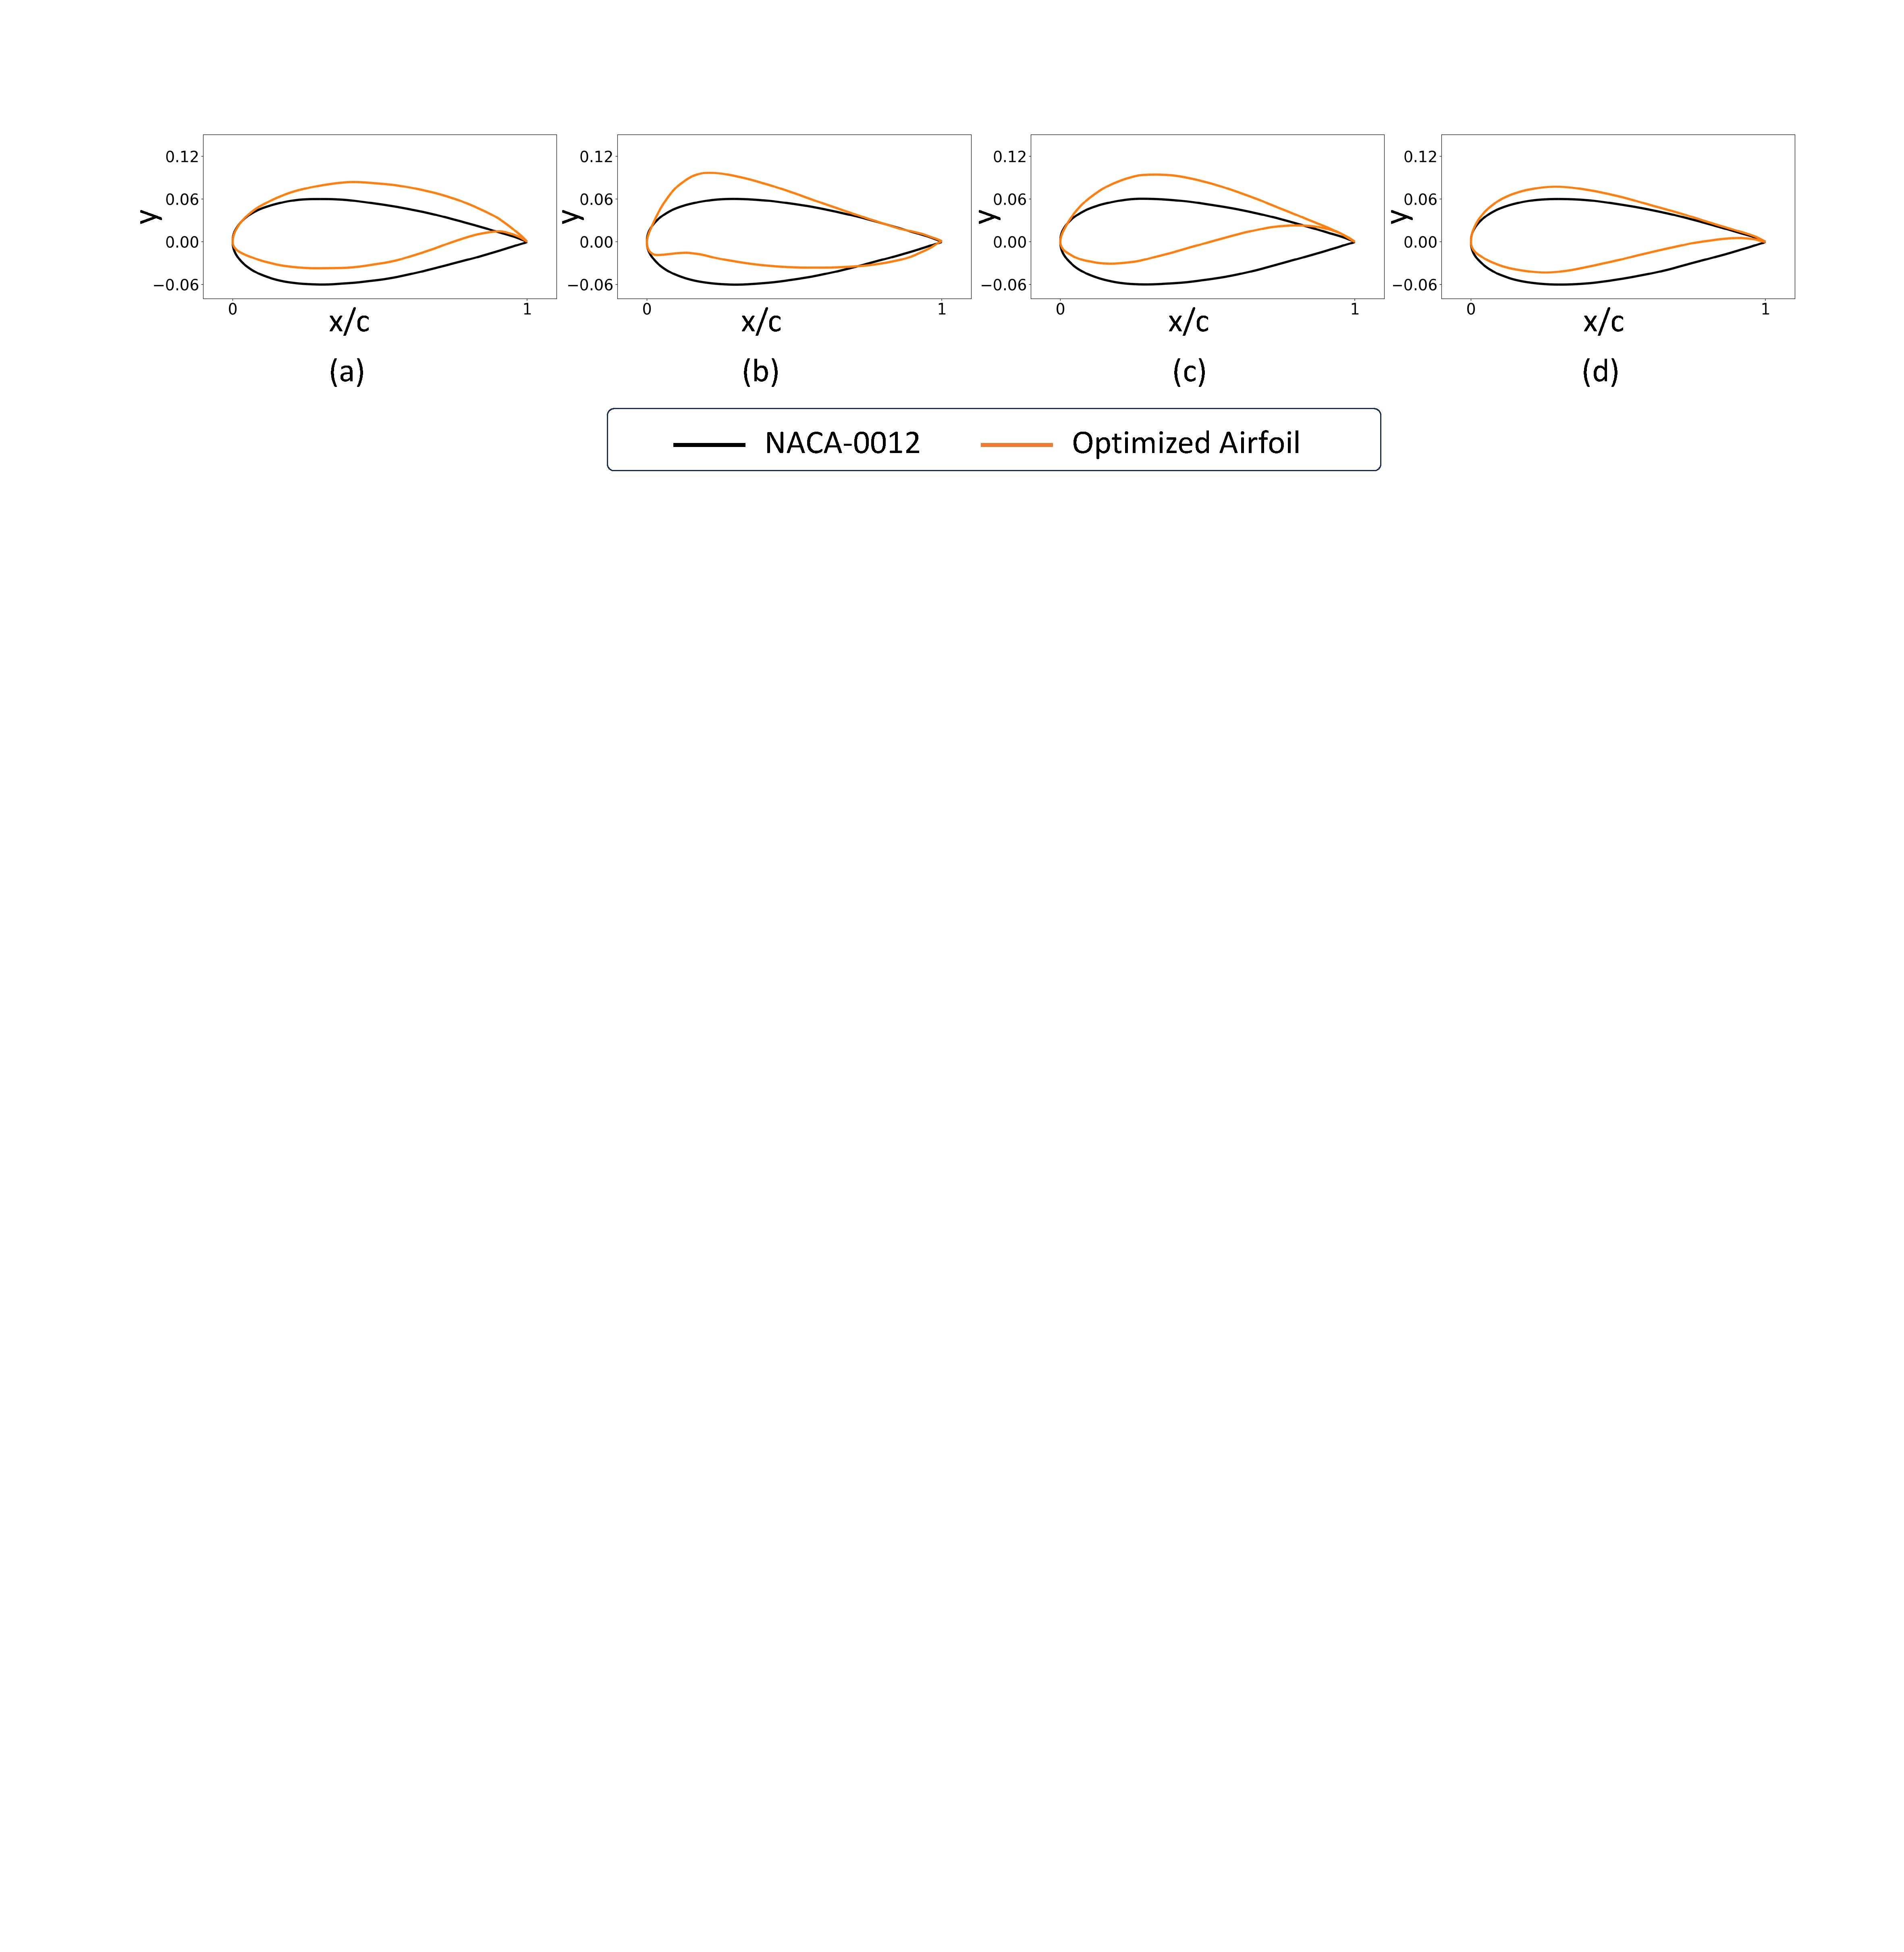
\includegraphics[width=1\linewidth]{chapter6/fig/SBO_optim_airfoil.pdf}
    \end{center}
    \caption{
        \small NACA-0012 baseline and optimized airfoils by (a) SM\#1-1, (b) SM\#1-2, (c) SM\#2, and (d) SM\#3.
    }
    \label{ch6:fig:main_SBO_optimized_airfoils}
\end{figure}

With these generated airfoils, we evaluate their aerodynamic performance using a triangulated CFD mesh built on NACA-0012\footnote{\scriptsize\url{https://github.com/su2code/Tutorials/blob/master/design/Inviscid_2D_Unconstrained_NACA0012/mesh_NACA0012_inv.su2}}. The \textit{DeepGeo} model ~\cite{aa.Wei2023b,aa.Wei2024b,aa.Wei2025} is used to deform this mesh to each dataset profiles. Flow simulations are conducted by the Euler solver in \textit{SU2}~\cite{aa.Economon2016}, providing the lift $C_L$ and drag $C_D$ coefficients. The airfoils and corresponding aerodynamic performance are used to train surrogate models that predicts $C_L$ and $C_D$. The surrogate is a simple multi-layer perceptron (MLP) consisting of two hidden layers with ReLU activations. The input features are 120-dimensional vectors concatenated from the $x$ and $y$ coordinates of $60$ points sampled from the airfoil contour. We train each surrogate model for 500 epochs using Adam optimizer to minimize mean squared error (MSE) between predictions and simulated $C_L$ and $C_D$ in the training set.

The shape optimization uses LSM and its latent space for parameterization. The latent code $\bz$ is first initialized by encoding the baseline NACA-0012 airfoil using Equation~\ref{ch6:eq:agmin_f_z}. We then perform gradient-based optimization on $z$ to maximize L/D subject to geometric and regularization constraints. The optimization problem is:
\begin{equation}
    \bz^* = \argmin_\bz ||C_D(\bz)||^2 - ||C_L(\bz)||^2 + C^I_{MT}(V) + w_\bz||\bz||^2\;,
\end{equation}
where $\{C_D(\bz), C_L(\bz)\}$ are the lift and drag predicted by the surrogate for the shape corresponding to latent $z$. The term $w_z||z||^2$ with a small weight $w_z$ prevents the optimizer from being far from the latent manifold and penalizes extremely large latent perturbations. We use the Adam optimizer on $z$ with a learning rate of $10^{-4}$ and $2000$ iterations to ensure convergence.

\begin{table}[htbp]
  \centering
  \caption{Surrogate-based optimization results and surrogate model accuracy ($R^2$).}
  \resizebox{\textwidth}{!}{
    \begin{tabular}{l|ccc}
    \hline
    \textbf{Surrogate Model} & \textbf{Final Surrogate $L/D$} & \textbf{Final Simulation $L/D$} & \textbf{Surrogate Model Accuracy (R2 Score)} \\
    \hline
    SM\#1-1 & 6.4322  & 6.6236  & 0.3265  \\
    SM\#1-2 & 1.2432  & 0.9195  &-2.1509  \\
    SM\#2 & 4.8718  & 5.8405  & 0.2041  \\
    SM\#3 & \textbf{8.2603}  & \textbf{7.7188}  & \textbf{0.9620}  \\
    \hline
    \end{tabular}%
  }
  \label{ch6:tab:main_SBO_results}%
\end{table}%

\subsubsection{Results}
Fig.~\ref{ch6:fig:main_SBO_optimized_history} shows the optimization histories with L/D versus iteration for each surrogate model. SM\#3, one relies on \textit{DiffGeo}, achieves the highest optimized L/D. Starting from the baseline L/D around 0.6, SM\#3's curve rises steadily to around 7.7 by 1200th iteration and plateaus. In contrast, SM\#1-1 and SM\#1-2 both show problematic behaviors: SM\#1-1 improves to around 7.5 L/D but then drops, while SM\#1-2 actually brings no improvement in true L/D. The wide-range sampling of SM\#1-2 clearly misled the surrogate model. SM\#2 performs better than SM\#1-1 but worse than SM\#3. These results show that surrogate models trained on \textit{DiffGeo}’s conditional samples guide the optimization to an improved design, whereas surrogates trained on random or mismatched data either plateau early or produce false optima that are not valid under CFD verification, highlighting that the quality of training data is critical.


To quantify surrogate fidelity, Table~\ref{ch6:tab:main_SBO_results} reports the $R^2$ score of each surrogate model measured by comparing surrogate-predicted L/D to CFD-simulated L/D along the optimization path. SM\#3 reaches an $R^2$ of $0.96$, showing its near-perfect consistency with simulated performance. SM\#3's prediction can be trusted throughout the optimization. By contrast, SM\#1-1, SM\#1-2 and SM\#2 show much lower $R^2$ scores (0.33, –2.15, and 0.20, respectively). An $R^2$ near 0 or negative indicates the surrogate was a very poor predictor of actual performance. These surrogate models can mislead the optimization, the true L/D only improved briefly, peaking around the 500-600th iteration, before declining as iterations continued. Since the surrogate prediction is the only indicator in real-world SBO applications, SM\#3's reliability is critical for practical deployment.

The final optimized shapes are compared in Fig.~\ref{ch6:fig:main_SBO_optimized_airfoils}. These four surrogate models produce distinctly different results. SM\#1-1, SM\#1-2 and SM\#2 generate airfoils with large cambers and aggressive deformations that lead to excessive drag and degraded actual performance. In contrast, SM\#3’s optimized airfoil is only a subtle modification of the baseline, yet achieves the highest L/D among all results. This result suggests that \textit{DiffGeo}’s samples helped the surrogate model generalize in the right region of design space around the baseline. 

It’s important to note that SM\#3’s advantage comes not only from generation in large numbers, but also from generating effective shapes. Both SM\#1 and SM\#3 used 500 samples, but SM\#1 random sampling produced most physically unrealistic or irrelevant geometries, bringing limited benefits to surrogate models. \textit{DiffGeo}, on the other hand, focused the sampling within a feasible domain through thickness conditioning. As a result, SM\#3 provided the surrogate model with more informative data that contains a diverse set of feasible and distinct airfoils that respect constraints while exploring meaningful shape variations. The improved optimization trajectory and final design quality observed with SM\#3 are direct consequences of both the precision and controllability of \textit{DiffGeo}'s energy-based guidance.

\subsubsection{Conclusions}

This SBO study demonstrates the practical value of \textit{DiffGeo} in a design loop and addresses the research questions posed at the start of this section.

\begin{itemize}
    \item[1.] \textbf{Data Efficiency:} \textit{DiffGeo} enabled high-quality, constraint-aware sampling and produced effectively produced 500 new designs that were more useful for the task than naive random perturbations or arbitrary historical designs when trained on only 50 unrelated airfoils.

    \item[2.] \textbf{Deployment Flexibility:} This case study shows that one can repurpose \textit{DiffGeo} to generate training data for a new optimization goal without retraining the generative model. The geometry–performance disentanglement showcase how a pretrained \textit{DiffGeo} can accelerate different design tasks with minimal effort.

    \item[3.] \textbf{Constraint Handling:} \textit{DiffGeo}’s guidance-driven sampling targets the feasible design space more effectively than conventional methods. Neither pure random sampling (SM\#1) nor arbitrary database collection (SM\#2) can easily incorporate such fine-grained constraints without manual filtering.
\end{itemize}

In summary, integrating \textit{DiffGeo} into the SBO pipeline can improve surrogate model's accuracy and guide optimization converged to a better design based on limited training data, eventually improving the efficiency and reliability of the design optimization.